% ------------------- PESW Template ------------------------------- %
\documentclass[conference, onecolumn, a4paper]{IEEEtran}

% -------------- Double Column Template --------------------------- %
%\documentclass[conference]{IEEEtran}
%\IEEEoverridecommandlockouts


% The preceding line is only needed to identify funding in the first footnote. If that is unneeded, please comment it out.
\usepackage{amsmath,amssymb,amsfonts}
\usepackage{algorithmic}
\usepackage[backend=biber]{biblatex}
\usepackage{graphicx}
\usepackage[american]{babel}
\usepackage{subcaption}
\usepackage{textcomp}
\usepackage{xcolor}
\addbibresource{bibliography.bib}
\def\BibTeX{{\rm B\kern-.05em{\sc i\kern-.025em b}\kern-.08em
    T\kern-.1667em\lower.7ex\hbox{E}\kern-.125emX}}


\begin{document}

\title{Assessment of a MACsec-based Security System for Use in Critical Infrastructure Communication}

\author{\IEEEauthorblockN{Lukas F{\"u}reder, Prof. Dr. J{\"u}rgen Mottok}
    \IEEEauthorblockA{\textit{Technical University of Applied Sciences Regensburg (OTH)} \\
        \textit{Laboratory for Safe and Secure Systems (LaS³)}\\
        Regensburg, Germany \\
        \{lukas.fuereder, juergen.mottok\}@oth-regensburg.de}
    \vspace{6 pt}
}

\maketitle

%%%%%%%%%%%%%%%%%%%%%%%%%%%%%%%%%%%%%%%%%%%%%%%%%%%%%%%%%%%%%%          Abstract           %%%%%%%%%%%%%%%%%%%%%%%%%%%%%%%%%%%%%%%%%%%%%%%%%%%%%%%%%%%
\begin{abstract}
    \noindent This paper investigates the integration of Media Access Control Security (MACsec) into the communication of critical infrastructure, 
    specifically within power grid applications, such as Substation Automation Systems (SAS) using the IEC 61850 standard. Building on the principles 
    of both standards, this study aims to determine if MACsec can meet the security and performance requirements set by IEC 62351 for power system 
    communications.
    
    \smallskip
    \noindent Furthermore, a  test environment containing a number of Intelligent Electronic Devices (IEDs) supporting communication compliant to all 
    IEC 61850 message types is established to evaluate this integration. The results of the measurements executed in this environment indicate that 
    MACsec could secure all types of messages, such as Manufacturing Message Specification (MMS), Sampled-Value (SV) and Generic Object Oriented 
    Substation Events (GOOSE), within the required time periods without significant delays. Even with additional encryption activated in the cipher suite, 
    the resulting transmission times are well below the required times. This suggests that MACsec can enhance the security goals for industrial 
    communication by providing confidentiality in addition to the already mandated assurance of authenticity and integrity to all messages without 
    compromising performance.

    \smallskip
    \noindent Only the requirement for end-to-end security cannot be met by MACsec in this configuration, as the security system re-encrypts with every 
    hop of the transmission. For this reason, we propose a hybrid approach of Transport Layer Security (TLS) and MACsec as part of future work. 
\end{abstract}
%%%%%%%%%%%%%%%%%%%%%%%%%%%%%%%%%%%%%%%%%%%%%%%%%%%%%%%%%%%%%%%%%%%%%%%%%%%%%%%%%%%%%%%%%%%%%%%%%%%%%%%%%%%%%%%%%%%%%%%%%%%%%%%%%%%%%%%%%%%%%%%%%%%%%%

\vspace{6 pt}

\begin{IEEEkeywords}
    MACsec, IEC61850, IEC62351, GOOSE, Secure Communication
\end{IEEEkeywords}

%%%%%%%%%%%%%%%%%%%%%%%%%%%%%%%%%%%%%%%%%%%%%%%%%%%%%%%%%%%%%%      Start of the Text      %%%%%%%%%%%%%%%%%%%%%%%%%%%%%%%%%%%%%%%%%%%%%%%%%%%%%%%%%%%
\section{Introduction}
\label{chapter:introduction}
\noindent The steady progress of digitalization is creating many new opportunities for society, business and science. However, this increasing connectivity 
especially among system relevant institutions and companies is also creating new challenges and potential threats. Companies classified as critical infrastructure, 
for example water supply facilities, power plants and their corresponding distribution systems, can constitute an attractive target for cyber attacks, 
which could disrupt the supply of basic resources to entire countries. As a result, laws such as the Network and Information Security Act (NIS-2) 
\cite{NIS-2:2022} of the European Union or the IT Act 2.0 \cite{IT-Gesetz_2:2021} enforced by the German Federal Office for Information Security (BSI) 
demand a unified level of cybersecurity for these entities. In these regulations, the councils prescribe that the companies must adhere to information 
security standards, which mandate the current requirements for secure communication and cryptography \cite[p. 9]{BSI-ISMS:2017}. Furthermore, the 
extension of the IT Act 2.0 dictates that these companies are obliged to provide proof of compliance with the security requirements over a two-year 
period \cite[§11 (1e)]{IT-Gesetz_2:2021}. This decision is intended to ensure the future operability of the security systems with respect to adapting 
changes of the latest technologies. 

\smallskip
The main objectives of these security standards are the assurance of the security goals authenticity, integrity and confidentiality for applications in 
critical infrastructure \cite[§2 (13)]{IT-Gesetz_2:2021}. Organizations such as the International Electrotechnical Commission (IEC) or the Institute of 
Electrical and Electronics Engineers (IEEE) develop standards that specify the implementation of these abstract security goals. This paper evaluates the 
currently established implementation of protection systems securing communication in Substation Automation Systems (SASs) and thereby provides a brief 
overview of the communication standards used in these facilities. Following this, we propose a Media Access Control Security (MACsec) based security system 
and evaluate whether this implementation fulfills the requirements of the security goals specified in the IEC 62351 security standards. 

\smallskip
The further course of the paper is structured as follows: Chapter \ref{chapter:fundamentals} clarifies the technical background of this paper and thereby 
provides a general overview of the IEC 61850 communication standard and the associated  message types. Building on this, the further part of this chapter 
presents the current state of message security mandated by the IEC 62351 security standard. Following this, a brief introduction into the MACsec security 
standard is provided, which presents the relevant features used in the implementation later on. Chapter \ref{chapter:relatedWork} displays relevant 
information presented by related work assessing the current state of technology in this topic. In the further course of the paper, Chapter 
\ref{chapter:implementation} explains the test setup used to measure the efficiency of the MACsec-based security system. In chapter \ref{chapter:evaluation} 
the data gathered is evaluated and placed in the context of the mandated security requirements. 

%%%%%%%%%%%%%%%%%%%%%%%%%%%%%%%%%%%%%%%%%%%%%%%%%%%%%%%%%%%%%%        Fundamentals         %%%%%%%%%%%%%%%%%%%%%%%%%%%%%%%%%%%%%%%%%%%%%%%%%%%%%%%%%%%
\section{Background}
\label{chapter:fundamentals}

\subsection{Overview of the IEC 61850 Standard}
\label{subchapter:IEC61850}
Among other standards used for communication in industrial applications, power systems primarily utilize the IEC 61850 standard \cite{IEC61850:2023}, 
which is published and maintained by the International Electrotechnical Comission (IEC) \cite{IEC61850_Overview:2006}. This standard specifies the 
transmission of diagnostic information, measurement values or control signals among devices structured in a hirachical three level architecture 
\cite{SGRWin_IEC61850Architecture:2021}, as displayed in Figure \ref{image:IEC61850Architecture}. The major advantage with this type of communication consists 
of the object-oriented data structure defined in this standard, which makes the integration of various components developed by different vendors possible 
\cite[p. 5643]{Review_IEC62351:2019}. 

\begin{figure}[h]
    \centering
    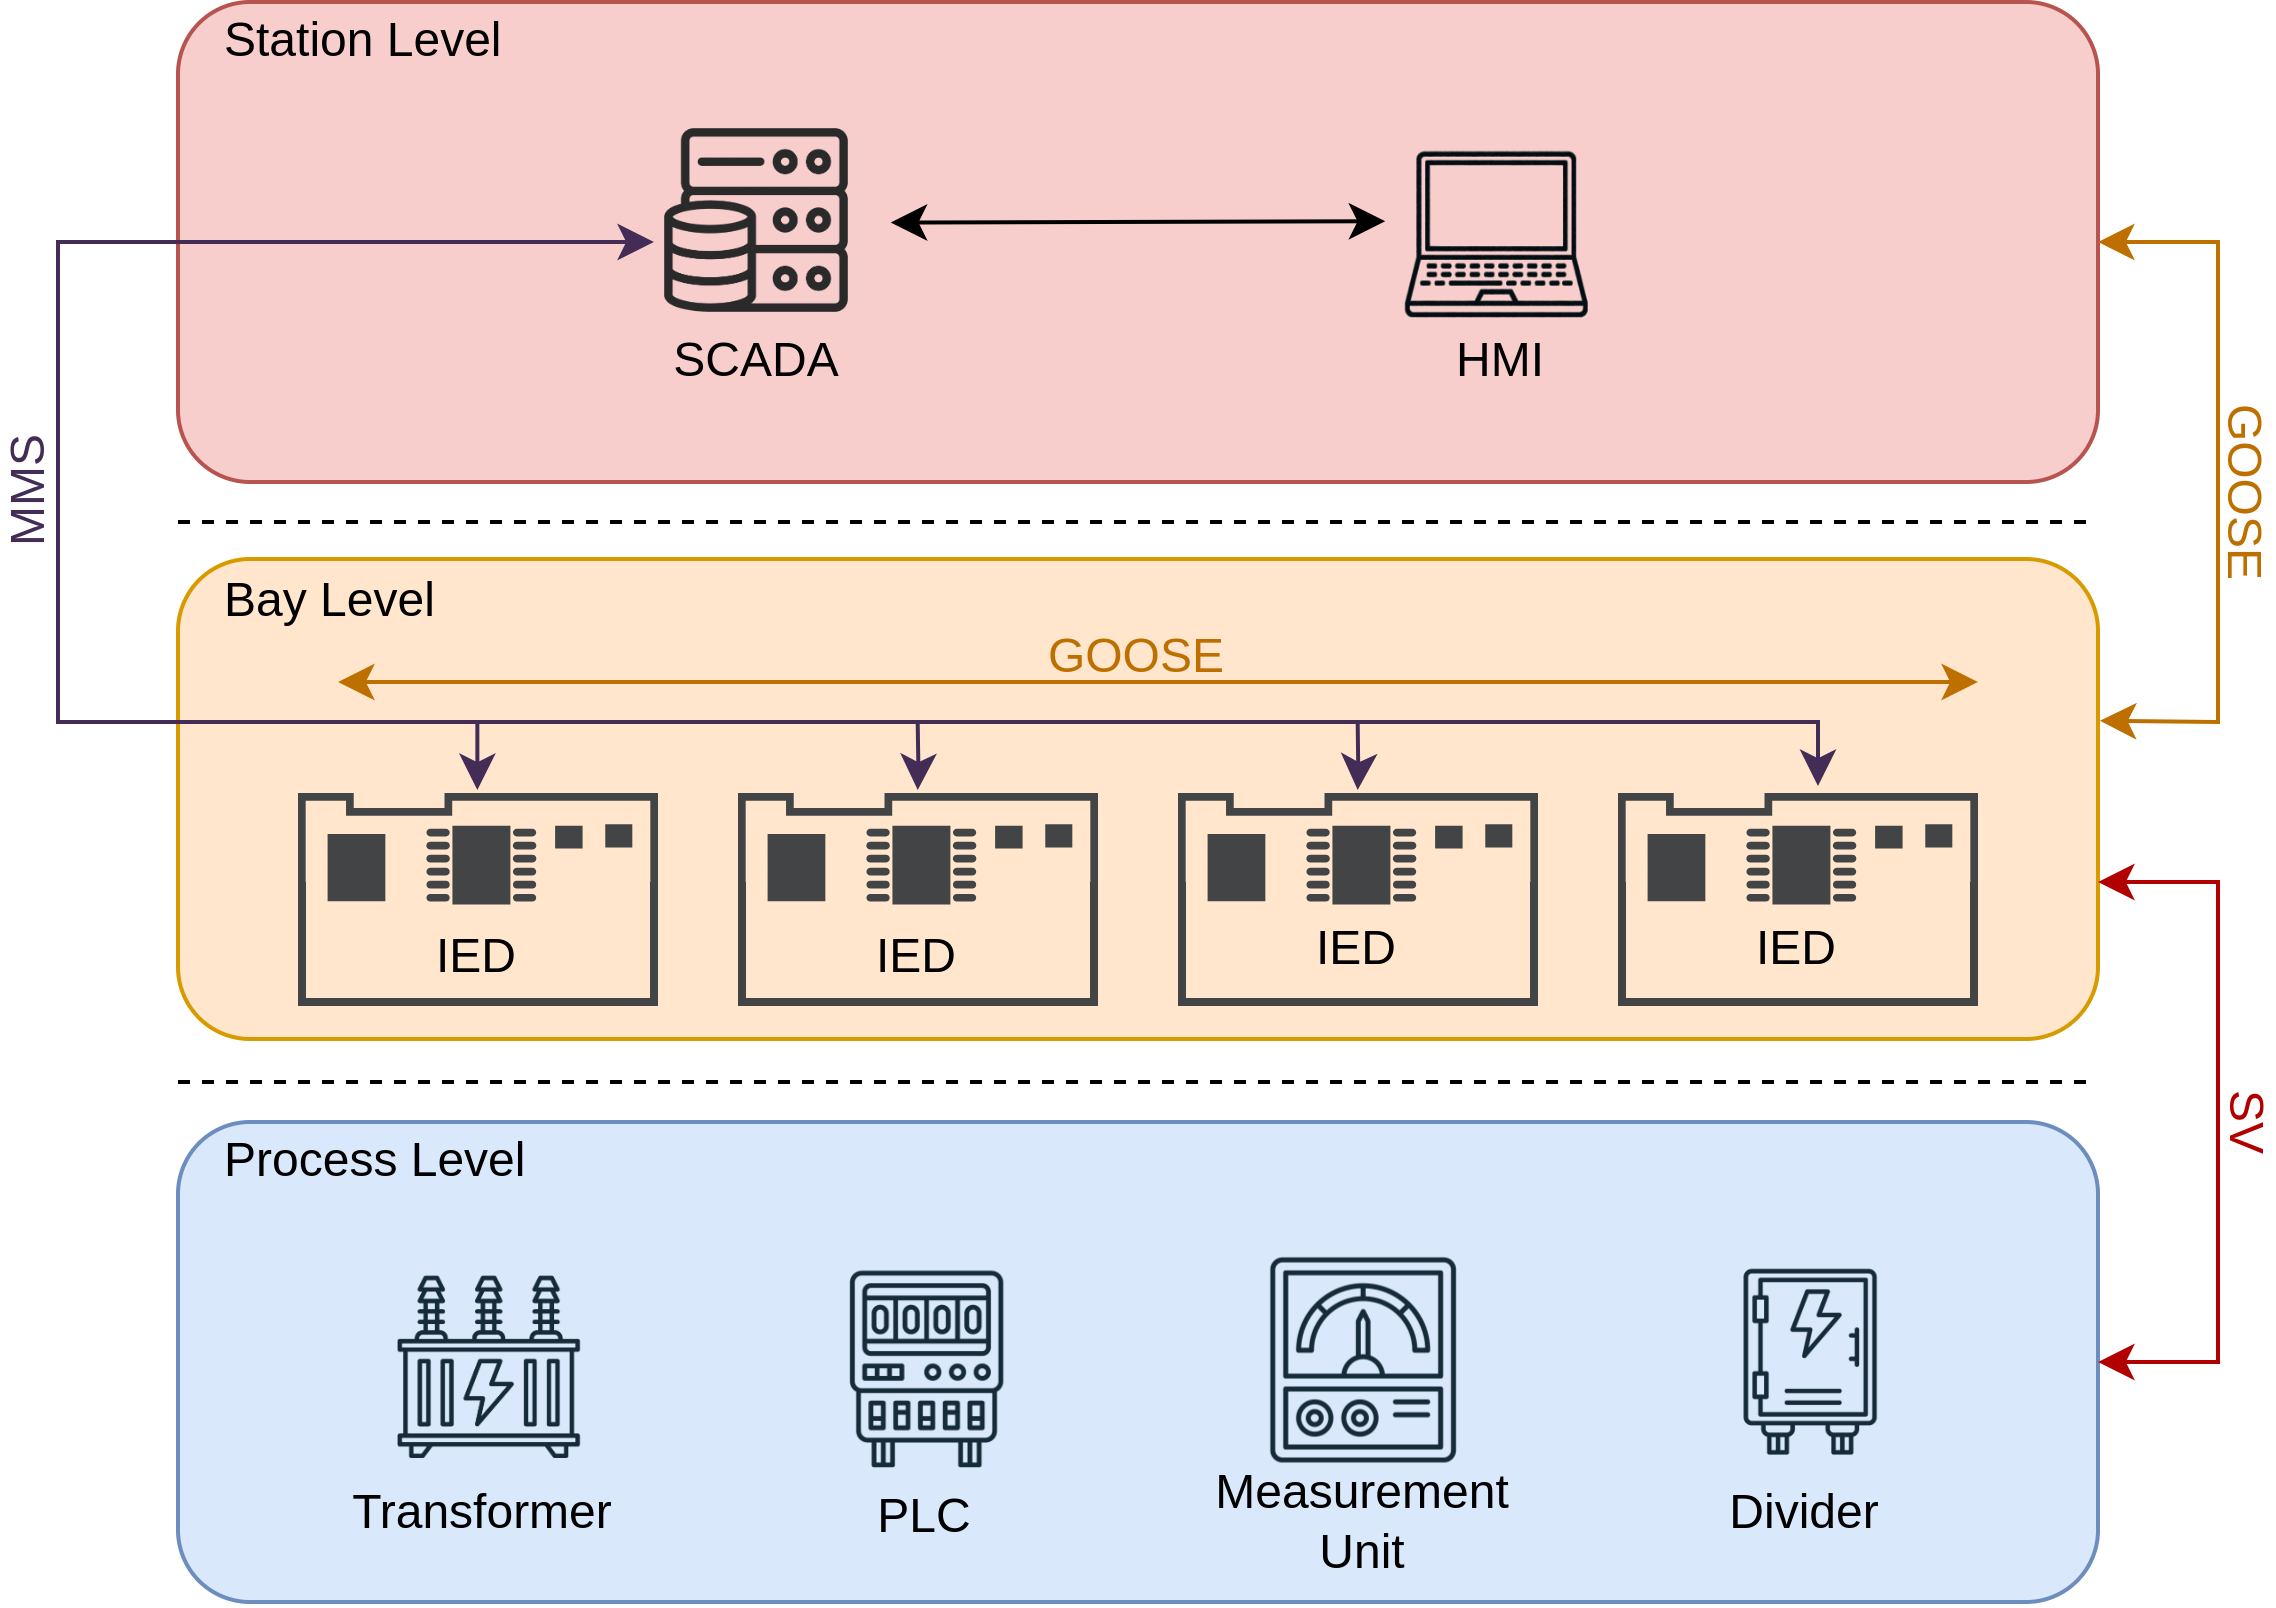
\includegraphics[width=0.65\textwidth]{images/IEC61850_Architecture.png}
    \caption{Overview of the three architecture levels in IEC 61850 \cite{SGRWin_IEC61850Architecture:2021}}
    \label{image:IEC61850Architecture}
\end{figure}

\noindent Closest to the powerlines, the \textit{Process Level} contains devices tasked with the actual power regulation. Examples for these are: transformers, 
circuit breakers, Programmable Logic Controllers (PLCs) and measurement units \cite{SGRWin_IEC61850Architecture:2021}. Upon configuration, Process Level 
components periodically publish measurement information to all subscribing communication partners in the Bay Level via Sampled-Value (SV) packets 
\cite{TyphoonHIL_IEC61850SV:2021}. This communication involves LAN-internal multicast packets, which take place exclusively on the second layer 
(Data Link Layer) of the Open System Interconnection (OSI) model \cite{TyphoonHIL_IEC61850SV:2021}. 

\smallskip
The \textit{Bay Level} above contains the Intelligent Electronic Devices (IEDs), each of which represents a transformation field in the substation 
\cite[p. 29]{IEC61850-7-1:2011}. The IEDs gather the measurement data from the Process Level and initially process them. The resulting information 
is then communicated through Manufacturing Message Specification (MMS) packets to other IEDs and the Station Level components \cite[p. 44]{IEC61850-8-1:2011}. 
Simultaneously, the IEDs receive control signals from the Station Level, which are also transmitted via MMS packets \cite{trafficGen_IEC61850:2011}. 
As the Station Level components are not necessarily located in the same LAN as the IEDs, the MMS messaging is implemented through TCP packets on the 
fourth layer (Transport Layer) of the OSI model \cite[p. 45]{IEC61850-8-1:2011}. In addition to the MMS messaging, the IEDs use Generic Object 
Oriented Substation Events (GOOSE) to send time-critical information to surrounding IEDs. Similar to SV, GOOSE messages are implemented on layer 2 if the OSI 
model through multicast Ethernet packets in the LAN \cite{GOOSE_confidentiality_integrity:2020}.

\smallskip
The devices located in the \textit{Station Level} of the architecture are responsible for controlling the SAS. This is achieved through MMS packets addressed 
to specific IEDs and the presentation of the processed information in graphical illustrations to the user \cite{SGRWin_IEC61850Architecture:2021}. 
For this, the Station Level components typically consist of a Supervisory Control and Data Acquisition (SCADA) component and a Human-Machine-Interface 
(HMI). As displayed in Figure \ref{image:IEC61850Architecture}, it is possible to transmit GOOSE messages to the Station Level components. 
For this, the IEC 61850-90-5 standard \cite{IEC61850-90-5:2012} defines a routable version of the layer two GOOSE frame. For this purpose, the GOOSE 
packets are extended by adding network and transport layer headers to form a UDP packet, which can be routed through multiple hops in a Wide Area Network (WAN) 
\cite{routable_GOOSE_SV:2020}.

%----------------------------------------------------------------------------------------------------------------------------------------------------%
\subsection{Message Security according to IEC 62351}
\noindent Building on the IEC 61850 message types described in Chapter \ref{subchapter:IEC61850}, the IEC 62351 standard \cite{IEC62351:2024} dictates 
security goals and requirements for cybersecurity solutions. In order to evaluate the proposed MACsec solution for industrial applications, 
we need to assess the proposed security functions according to the demands of this standard.

\smallskip
With regard to MMS messages, the standard prescribes the protection of authenticity, integrity and confidentiality. IEC 62351-4 directly specifies 
certificate-based TLS to achieve these security goals \cite{SecureMMS:2020}. Furthermore, the standard subdivides the assertion of the security requirements 
according to the layers of the OSI reference model. The upper three layers are summarized in the application profile and the lower four layers in the 
transport profile \cite{SecureMMS:2020}. Based on this, the standard specifies that the security system shall verify the authenticity of the communication 
partner and the integrity of the transmitted messages during the handshake phase of the transport profile \cite{Review_IEC62351:2019}. Following this, 
the system shall provide confidentiality for the outgoing messages in the data transfer phase \cite{SecureMMS:2020}. With respect to the upper three 
layers, the standard specifies two possible implementations in the application profile: peer-to-peer security and end-to-end security 
\cite{Review_IEC62351:2019}. The primary difference between them consists in the data origin authentication and message integrity checks, which are only 
verified during the association establishment in the peer-to-peer implementation, whereas the end-to-end implementation also ensures them in the following 
data transfer \cite{Review_IEC62351:2019}.

\smallskip
For GOOSE messages, the standard argues that the strict real-time requirement of a maximum of 3 ms \cite{GOOSE_confidentiality_integrity:2020} outweighs 
the security requirements and for this reason, state that security measures which affect the transmission rates are not acceptable \cite{PoisonedGOOSE:2014}. 
Building on this, the IEC 62351 standard advises against the encryption of GOOSE messages and only proposes the use of digital signatures to verify the 
authenticity of the GOOSE publisher and the integrity of the message. As similar restrictions arise for SV messages, the standard equally advises the 
usage of digital signatures for SV packets \cite{Review_IEC62351:2019}. 

%----------------------------------------------------------------------------------------------------------------------------------------------------%
\subsection{Fundamentals of the MACsec Security Standard}
\noindent MACsec represents an information security standard which protects messages on the second layer (Data Link Layer) of the OSI model. In contrast 
to security standards operating in higher layers of the TCP/IP stack (e.g. TLS), which provide end-to-end encryption, MACsec verifies the confidentiality, 
integrity and authenticity of a packet within each hop of the transmission \cite{Cybersecurity_Substation:2016}. However, this lower layer implementation 
close to the PHY enables MACsec to secure communication which takes place exclusively on layer 2 (e.g. SV \& GOOSE). The following paragraph explains the 
most important aspects of the MACsec standard, which are responsible for ensuring the authenticity, integrity and confidentiality of the transmitted packets.

\begin{figure}[h]
    \centering
    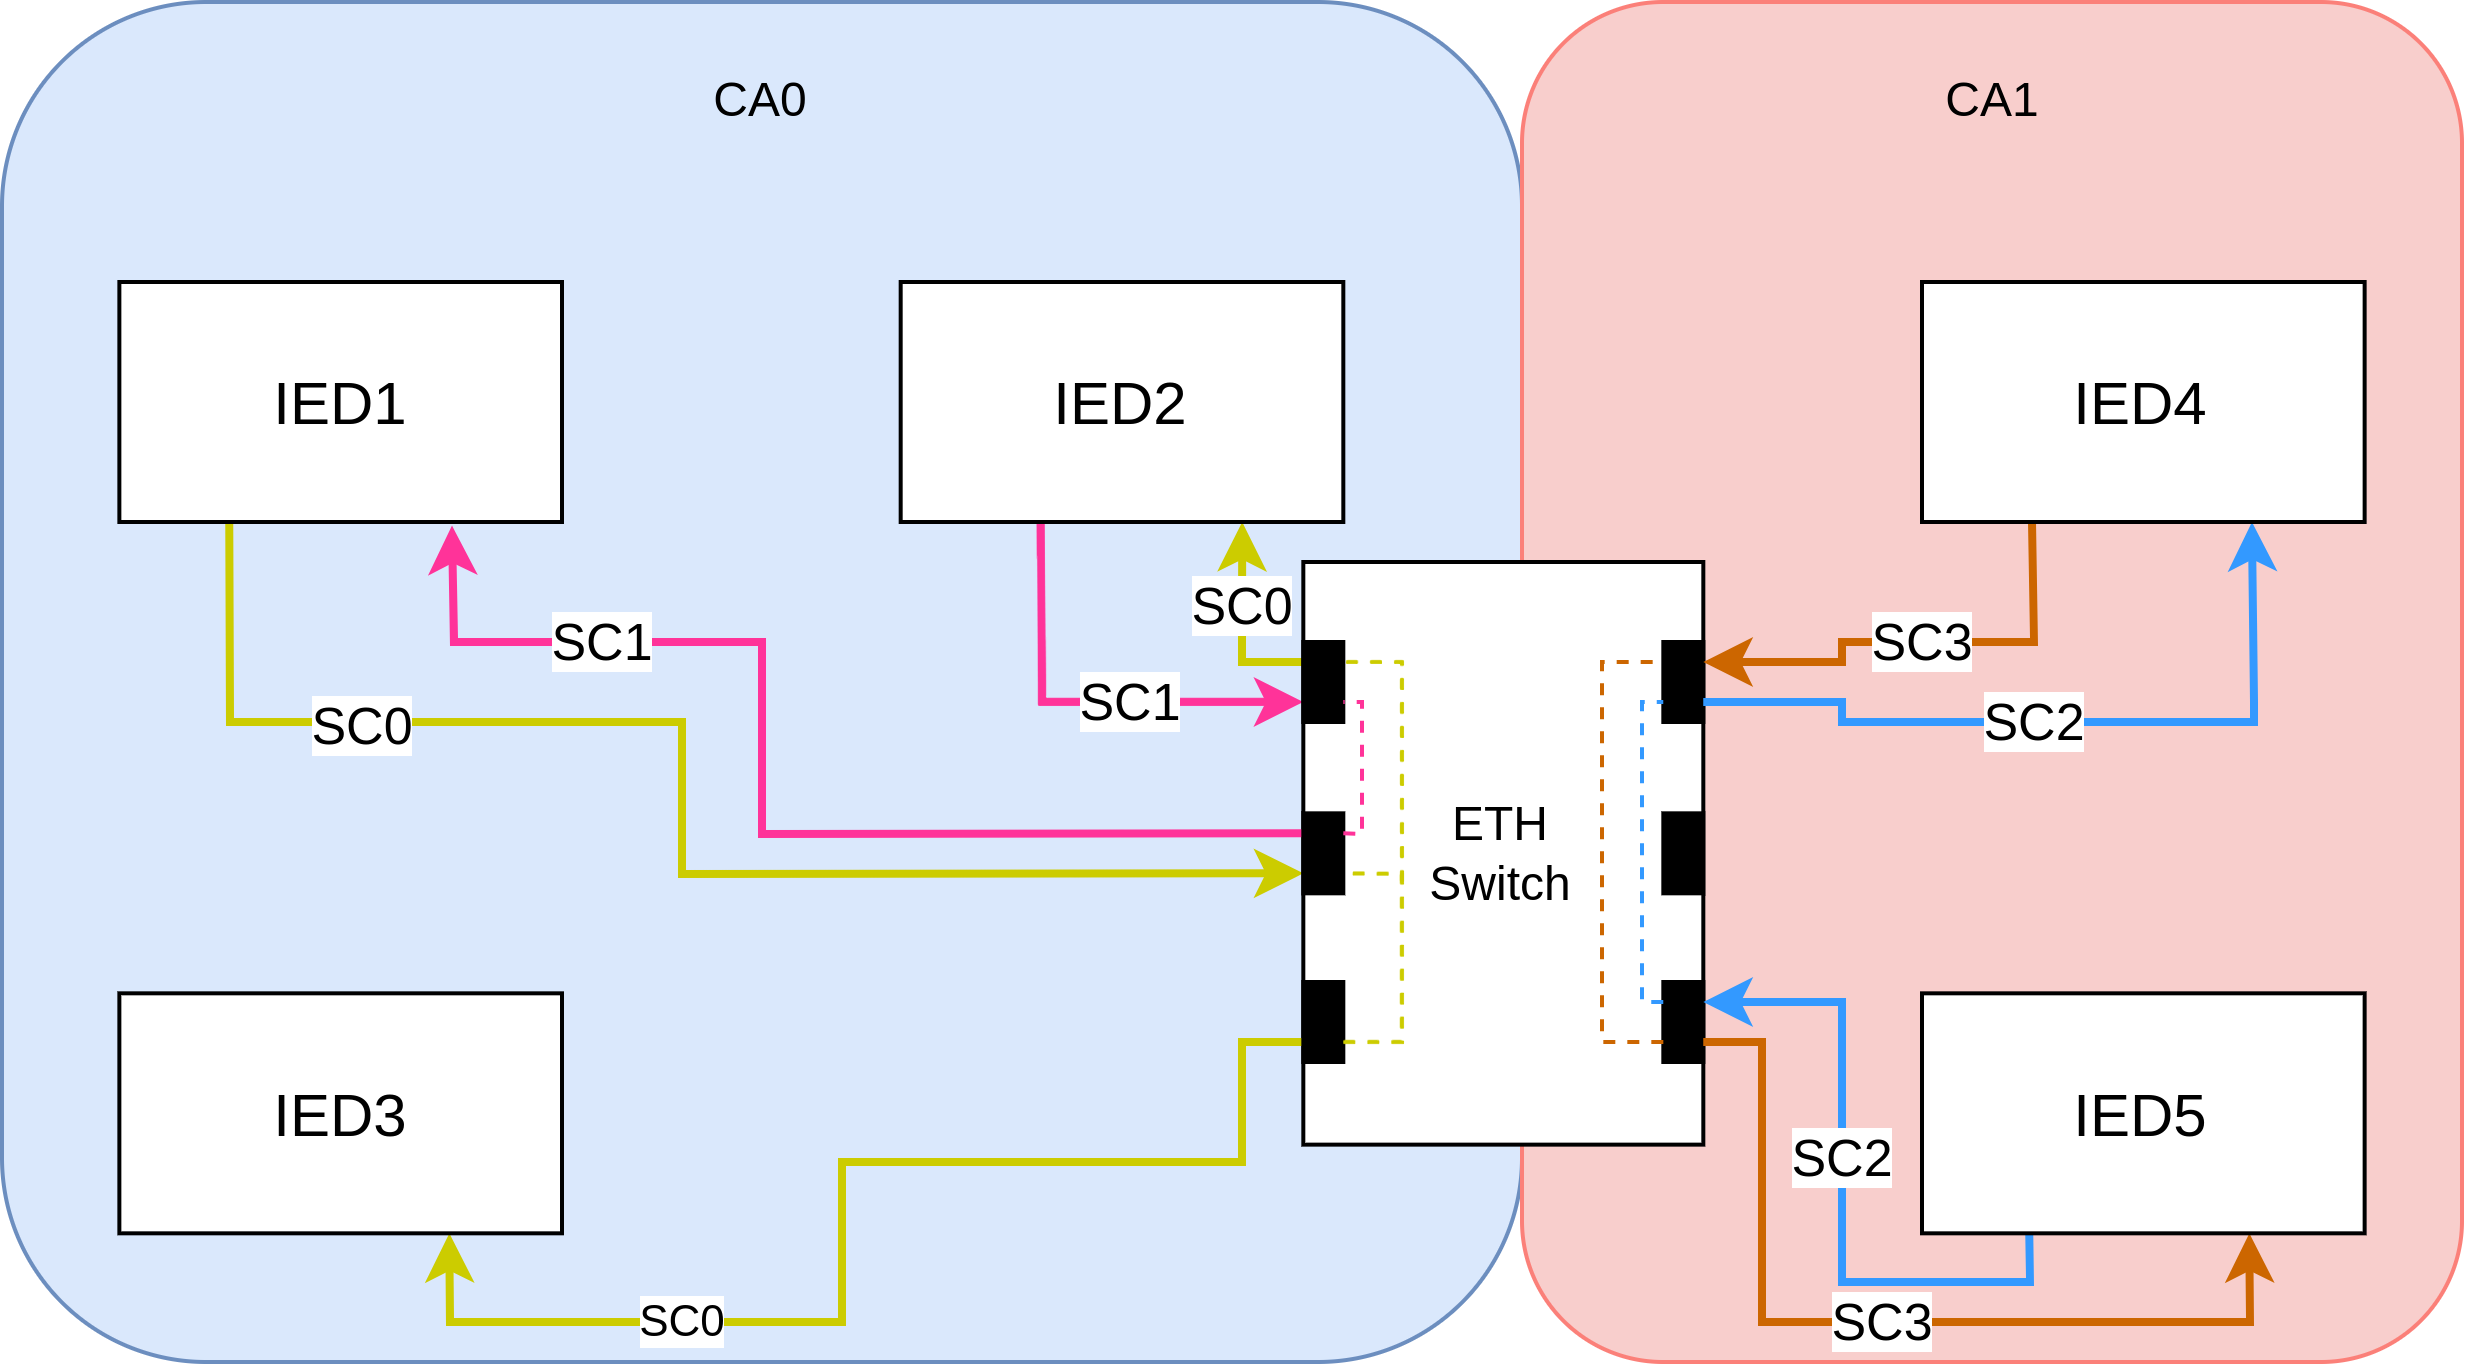
\includegraphics[width=0.65\textwidth]{images/MACsec_Entities_Diagram.png}
    \caption{Schematic representation of the MACsec entities \cite{IEEE-802-1AE:2018}}
    \label{image:MACsecEntities}
\end{figure}

\noindent As displayed in Figure \ref{image:MACsecEntities}, the communicating devices are initially grouped into Connectivity Associations (CAs), which 
represent the logical separation of secured communication areas \cite[p. 35]{IEEE-802-1AE:2018}. Each member of a CA possesses the associated Connectivity 
Association Key (CAK), which is later used to generate the individual session keys. Similar to other encryption systems, the CAK acts as a shared 
secret between the individual parties and is therefore used to verify the authenticity of of other devices in the same CA. In the IEEE 802.1AE standard, 
the distribution of the CAK among the participants is only specified as a brief overview of the established methods \cite[p. 230]{IEEE-802-1AE:2018}. 
In our case, we utilize pre-shared keys to configure the CA in the test setup explained in Chapter \ref{chapter:implementation}. Within a CA, the 
connections between the communicating devices are referred to as Secure Channels (SCs). As displayed in Figure \ref{image:MACsecEntities}, 
an SC is a unidirectional connection from a transmitter to one or more receivers. Each SC can be identified by the Secure Channel Identifier (SCI), 
which is added to the MACsec specific field in the secured frame \cite[p. 43]{IEEE-802-1AE:2018}. During transmission over an SC, the packets are sent 
within Security Associations (SAs). These are time intervals in which a single Secure Association Key (SAK) is valid \cite[p. 44]{IEEE-802-1AE:2018}. 
The SAK is the session key, which is derived from the previously described CAK and is only valid for up to ${(2^{32} -1)}$ packets, after which a new 
SAK needs to be generated \cite[p. 66]{IEEE-802-1AE:2018}. To be able to monitor the number of transmitted packets in an SA, the MACsec frame contains 
a packet number field, which is incremented with each subsequent packet. This field additionally ensures that no replay attacks can be carried out on 
the network \cite[p. 145]{IEEE-802-1AE:2018}. 

\smallskip
To ensure authenticity, confidentiality and integrity of the transmitted frames, MACsec utilizes Authenticated Encryption with Associated Data (AEAD) 
cipher suites. These encryption systems typically consist of a symmetric block cipher and a Message Authentication Code (MAC) generator 
\cite{NIST-AES_GCM:2007}. The first entity of which provides the option to encrypt the payload of the message, while the second entity simultaneously 
generates a MAC over the entire message \cite{GOOSE_confidentiality_integrity:2020}. For usage, the IEEE 802.1AE standard specifies four variations of 
the Advances Encryption System in Galois/Counter Mode (AES-GCM) \cite[p. 143ff]{IEEE-802-1AE:2018}.

%%%%%%%%%%%%%%%%%%%%%%%%%%%%%%%%%%%%%%%%%%%%%%%%%%%%%%%%%%%%%%        Related Work         %%%%%%%%%%%%%%%%%%%%%%%%%%%%%%%%%%%%%%%%%%%%%%%%%%%%%%%%%%%
\section{Related Work}
\label{chapter:relatedWork}
\noindent To assess the operating principle of a MACsec-based security system in IEC 61850 compliant communication, it is necessary to understand both 
the working method of the communication inside a substation as well as the corresponding functionality of the MACsec security standard. The following 
related work display these important aspects and are therefore relevant for the implementation of an experimental setup for MACsec secured industrial 
communication.

\smallskip
Mackiewicz \cite{IEC61850_Overview:2006} describes the overall usage of the IEC 61850 protocol by illustrating key features as well as the general aspects 
of IEC 61850 compliant communication. Since this standard represents a core part of the communication inside of power grid systems, it is vital to 
understand the corresponding aspects such as communication paths, model structures or data addressing in order to design a representative test environment. 

\smallskip
Hussain  \textit{et al.} \cite{Review_IEC62351:2019} published a paper assessing the IEC 62351 standard and its security mechanisms towards IEC 61850 
compliant messaging. The publication initially describes the basic values and security goals of the safety standard and, building on this, which attacks 
can potentially be carried out on IEC 61850 messages to manipulate the internal workings of a SAS. At this point, the paper primarily focuses on the 
Ethernet-based message types GOOSE and SV and the associated decision not to encrypt them due to strict real-time delivery requirements.  

\smallskip
Lackorzynski \textit{et al.} \cite{MACsecIndustrialOptimization:2020} proposed modifications of the IEEE 802.1AE standard to improve MACsec for usage 
in industrial applications. In particular, the fragmentation of Ethernet frames was considered. This procedure is necessary, if messages exceed the 
Maximum Transmission Unit (MTU) and are thus possibly discarded by the recipient of the message. The presented implementation ensures the adherence to 
to the MTU and splits messages into multiple frames if it is exceeded. Additionally, the authors discuss the usage of different cipher suits instead of 
the AES-GCM 128/256 specified in the MACsec standard. The evaluation of their study shows that the ChaCha20-Poly1305 cipher is a promising alternative 
for industrial applications.

\smallskip
Moreira \textit{et al.} \cite{Cybersecurity_Substation:2016} evaluate various approaches to introduce cybersecurity in SASs. Initially, a brief outline 
of the communication structures in substations is presented. Building on this, various established security approaches are explained and evaluated based 
on the protection objectives of the IEC 62351 standard. The authors also point out possible implementation problems, such as incompatibilities between 
the security systems and the communication protocols or the handling of redundant packets inside ring-topology networks. In the further course of the 
paper, the authors propose the idea of MACsec-based communication security in SASs and discuss the possible advantages and challenges that arise with it. 

\smallskip
Hussain \textit{et al.} \cite{GOOSE_confidentiality_integrity:2020} analyzed possible GOOSE security implementations based on their preceding review 
of the IEC 62351 standard \cite{Review_IEC62351:2019}. Especially concerning the decision to abstain from implementing confidentiality in GOOSE messages, 
the authors argue that the critical payload of these messages demand encryption to provide efficient protection against attacks. However, in order to 
meet the real-time requirements of the protocol, they suggest replacing the RSA signature with encryption using an AEAD cipher. In the further course 
of the paper, they compare encryption and signature times between different AEAD ciphers and conclude based on the measurement results that these encryption 
systems pose a promising solution, which provides the opportunity to encrypt the message while simultaneously  meeting the 3 ms timing requirement.

\smallskip 
Building on the theoretical proposition of Moreira \textit{et al.} \cite{Cybersecurity_Substation:2016}, we formulate our evaluation of MACsec for use in 
substations and other power systems based on the IEC 61850 standard. Along with this, we consider the findings of Hussain \textit{et al.} \cite{Review_IEC62351:2019} 
in relation to the proposed modifications of the security goals for Ethernet-based messaging in IEC 62351 for the implementation of our MACsec test environment. 
From this, our experimental setup enables us to discuss the advantages and disadvantages of MACsec in comparison with the security goals of the IEC 62351 
standard as well as the timing requirements of the IEC 61850 standard. 

%%%%%%%%%%%%%%%%%%%%%%%%%%%%%%%%%%%%%%%%%%%%%%%%%%%%%%%%%%%%%%       Implementation        %%%%%%%%%%%%%%%%%%%%%%%%%%%%%%%%%%%%%%%%%%%%%%%%%%%%%%%%%%%
\section{Implementation}
\label{chapter:implementation}
\noindent To display the communication in a SAS, we implement a test environment consisting of three Bay Level components. As the IEDs take part 
in all forms of message exchange inside the substation architecture, they are perfectly suitable for testing the communication in conjunction with MACsec. 
In order to ensure the reproducibility of this study, we decided to use the Raspberry Pi 4 as hardware platform for all devices in the setup. With respect 
to the software used in the applications, we utilize the open-source library libiec61850\footnote{source: https://libiec61850.com/} to establish the 
different communication types and data structures of the IEC 61850 standard. To integrate MACsec into the communication, we utilize the MACsec Linux kernel 
module\footnote{source: https://github.com/torvalds/linux/blob/master/drivers/net/macsec.c}, which establishes a configurable virtual interface on top of 
an existing network interface \cite{MACsecLinuxModuleDoc:2016}. For the implementation of the time measurement in Chapter \ref{subchapter:TestProcedures},  
we integrate the WiringPi\footnote{source: https://github.com/WiringPi/WiringPi} library into the project. This enables us to access peripherals of the 
hardware platform and results in precise time measurement across several communication participants. 

\smallskip 
The remainder of this chapter proceeds as follows: Chapter \ref{subchapter:TestEnvironmentStructure} initially explains the overall structure of the 
test environment. Chapter \ref{subchapter:TestEnvironmentMACsec} describes the optionally activatable MACsec configuration and the corresponding entities 
of the security standard. Chapter \ref{subchapter:TestProcedures} elaborates on the subsequent test executions and the transmission time measurement. 

\subsection{Structure of the Test Environment}
\label{subchapter:TestEnvironmentStructure}
\noindent As displayed in Figure \ref{image:MACsecTestSetup}, we configure IED1 as a publishing server and IED2 and IED3 as subscribing clients. 
Furthermore, the implementation of IED1 contains an XML data structure compliant to the specification of the Substation Configuration Language (SCL) 
in IEC 61850-6 \cite{IEC61850-6:2010}. This file contains the communication and processing information of the IED itself \cite{IEC61850_Overview:2006}.

\smallskip
In our case, we integrate a measurement unit (MMXU) \cite[p. 268]{IEC61850-7-4:2010} and a control unit (LLN0) \cite[p. 164]{IEC61850-7-4:2010} 
into the SCL file of IED1. During runtime, IED1 continuously populates the data points of the measuring unit with sampled values of a sinusoidal function. 
In addition to the actual measurement, each sampled value contains a time stamp and a quality index \cite[p. 61ff]{IEC61850-7-3:2010}. These values can 
then be requested by IED2 and IED3 via MMS messages.

\begin{figure}[h]
    \centering
    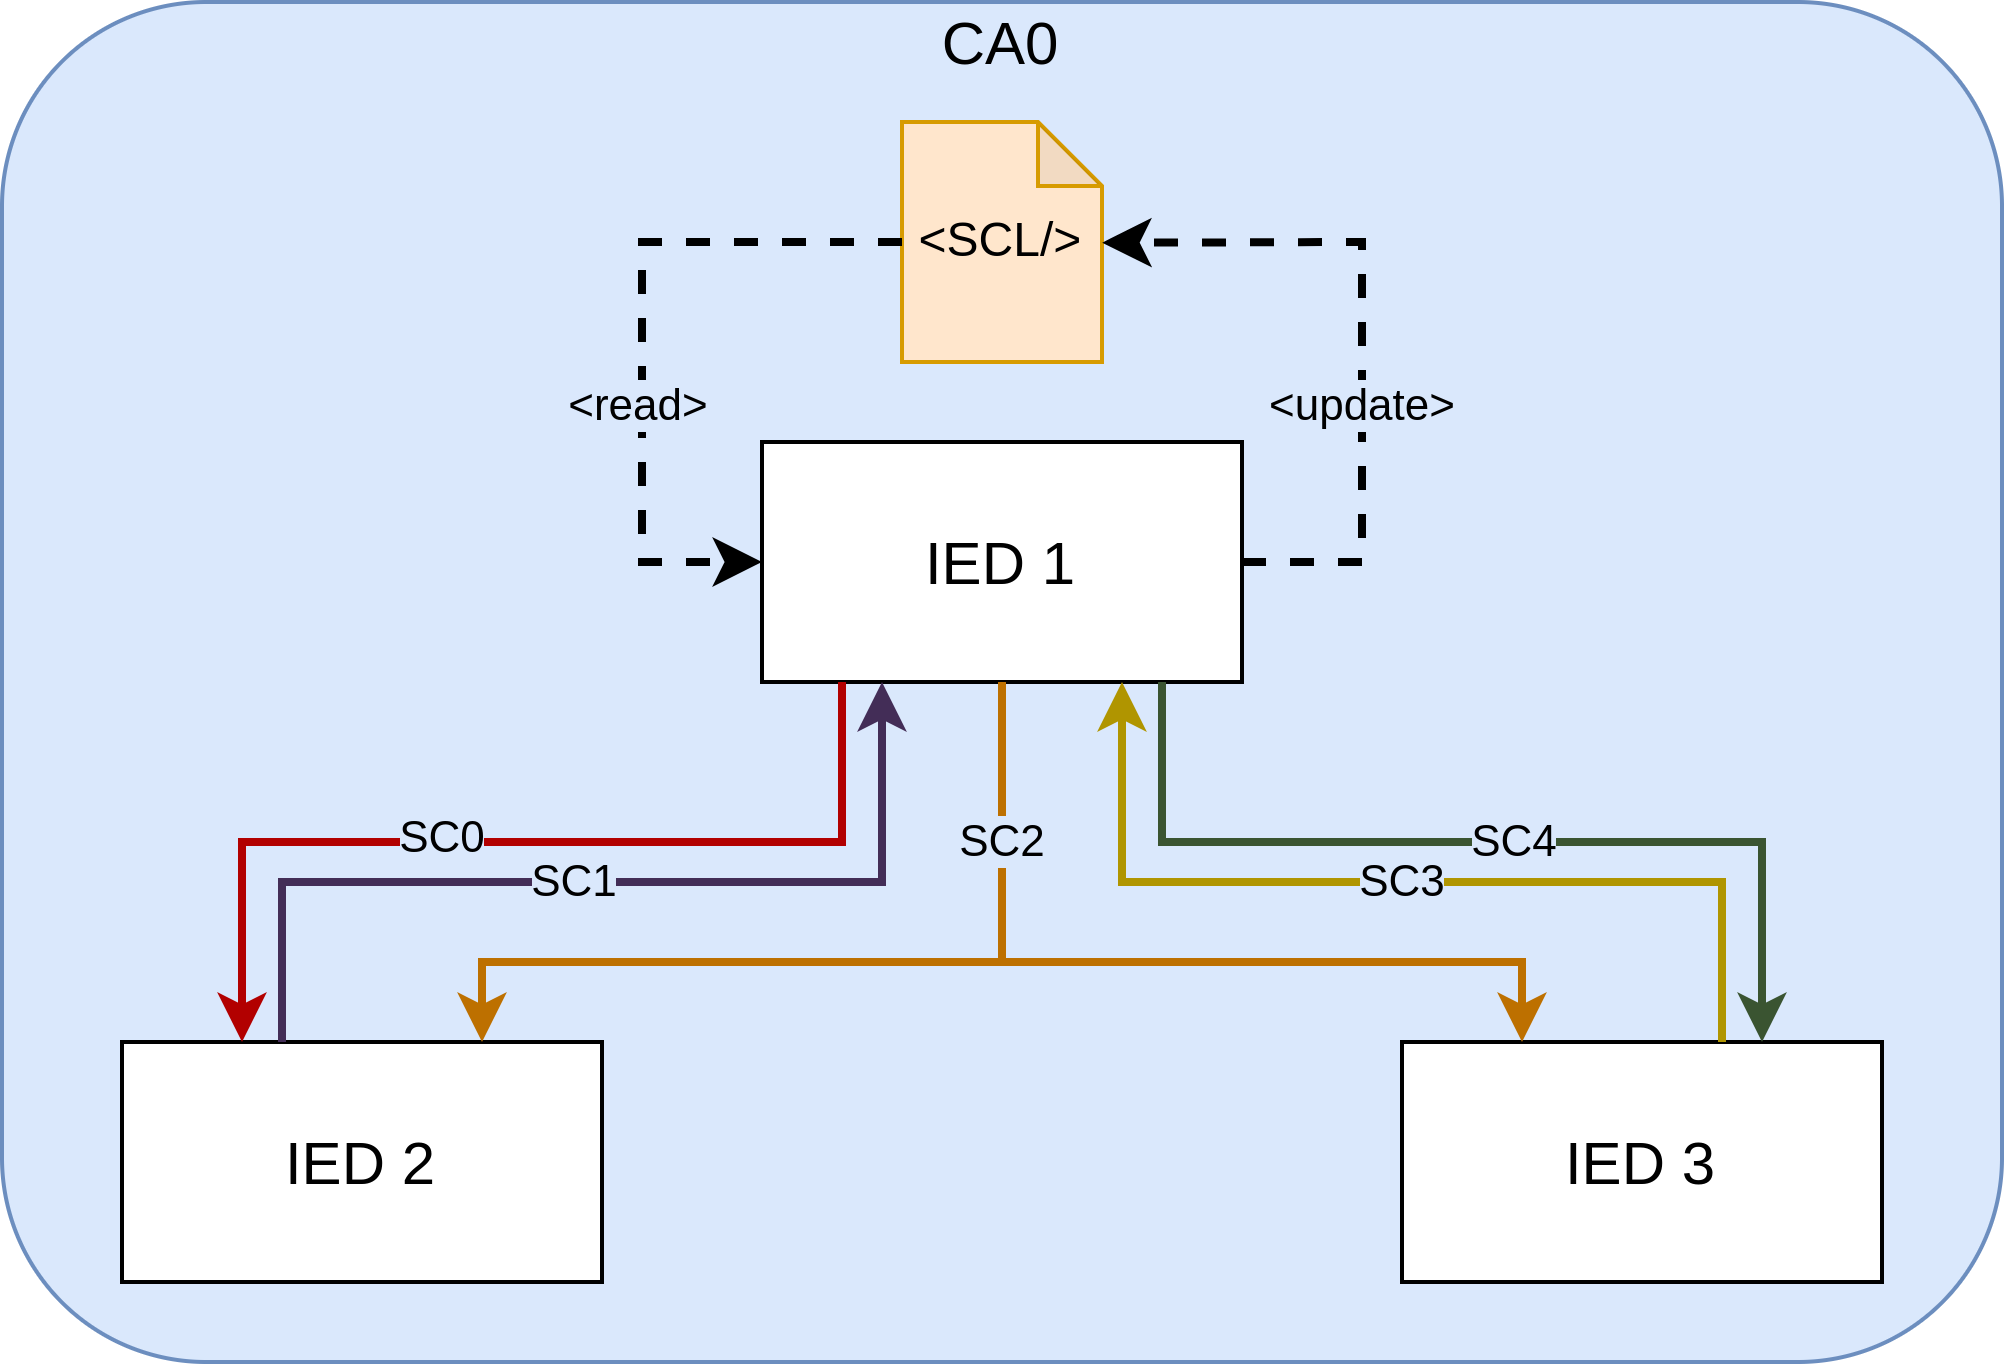
\includegraphics[width=0.55\textwidth]{images/TestSetupIEDs.png}
    \caption{Component Structure of the Test Setup}
    \label{image:MACsecTestSetup}
\end{figure}

\noindent In addition to the TCP request-response communication via MMS messages, IED1 periodically publishes GOOSE and SV messages in a configurable 
interval containing the current value of the measurement. The configuration of the GOOSE messages, which contains the corresponding multicast MAC address, 
VLAN ID and VLAN priority, are equally stored in the control unit of the SCL file \cite[p. 189]{IEC61850-8-1:2011}. For the transmission of the SV 
packets, an Application Protocol Data Unit (APDU) is configured during the initialization phase of the server. This object contains the floating-point 
value of the latest measurement and a message time stamp. As the application progresses, the content of the APDU is periodically updated and published. 
On the subscriber side, the subscription to the corresponding events (in this case GOOSE and SV) is implemented in software in the form of asynchronous 
handler functions, which subsequently log the incoming information. 

%----------------------------------------------------------------------------------------------------------------------------------------------------%
\subsection{MACsec integration in the Test Environment}
\label{subchapter:TestEnvironmentMACsec}
\noindent Building on the general structure of the test environment described in Chapter \ref{subchapter:TestEnvironmentStructure}, the implementation of 
MACsec into the test setup can now be explained. Initially, we integrate all devices in the same CA by distributing a pre-shared CAK. Based on this key, 
the various SCs and SAs can be established as shown in Figure \ref{image:MACsecTestSetup}. For bidirectional MMS communication between two IEDs, one SC is 
required for each communication direction. Using the example of packet exchange between IED1 and IED2, we have configured the secure channels SC0 and SC1 
for this purpose. Each of these channels derives its own SAK from the CAK and establishes a secure connection for the duration of the SA. The establishment 
of SC3 and SC4 is carried out identically for MMS communication between IED1 and IED3.

\smallskip
With regard to the secure publication of GOOSE and SV packets, we established an additional SC (displayed in Figure \ref{image:MACsecTestSetup} as SC2), 
which is connected to both IED2 and IED3. This configuration enables us to multicast the messages while simultaneously securing the payload and ensuring 
authenticity and integrity. Since the configuration of this test environment only allows the publication of GOOSE and SV packets originating from IED1, 
we only need one SC to secure them with MACsec. Consequently, if IED2 and IED3 are also meant to send secure multicast messages, two additional SCs must be 
configured.   

%----------------------------------------------------------------------------------------------------------------------------------------------------%
\subsection{Definition of the Test Procedures}
\label{subchapter:TestProcedures}
\noindent To evaluate whether this MACsec implementation fulfills the time requirements of the IEC 61850 standard, we conduct a measurement of the 
transmission times for each of the different message types. In order to achieve a precise time measurement, we expanded the implementation of the server 
and the client application to toggle a General Purpose Input/Output (GPIO) pin during transmission and reception of the associated frame type. 
By using an external logic analyzer, the times between the voltage level shifts can be measured. Since this measurement is performed by an external device, 
we do not need clock synchronization between the communication participants, which significantly reduces the implementation efforts of the measurement. 

%%%%%%%%%%%%%%%%%%%%%%%%%%%%%%%%%%%%%%%%%%%%%%%%%%%%%%%%%%%%%%         Evaluation          %%%%%%%%%%%%%%%%%%%%%%%%%%%%%%%%%%%%%%%%%%%%%%%%%%%%%%%%%%%
\section{Evaluation}
\label{chapter:evaluation}
\noindent Based on the implementation design explained in Chapter \ref{chapter:implementation}, a number of transmission time measurements can be 
executed. We compare the times in three different configurations in order to be able to investigate the temporal influence of the security module. 
The first step is to measure the transmission times without the security module active, followed by MACsec frame protection with integrity check and 
encryption and lastly solely with MACsec integrity check. These measurements are carried out in the following chapters for all IEC 61850 message types.

\smallskip
The further course of this chapter is structured as follows: Chapter \ref{subchapter:EvalGOOSESV} illustrates the measurement results for GOOSE and SV messages
and Chapter \ref{subchapter:EvalMMS} presents the results for MMS messages.

\subsection{Temporal Influence of MACsec on SV and GOOSE messages}
\label{subchapter:EvalGOOSESV}
\noindent For the GOOSE and SV measurement, IED1 was configured in the test setup so that the corresponding packets are published periodically at 
intervals of 500 ms. In the next step, the temporal delay to the handler function of the client side was measured. This measurement was then repeated 
1000 times without additional computational load for both configurations and is therefore under ideal conditions. The results of these measurements are 
displayed in Figures \ref{imgae:GOOSETimings} and \ref{image:SVTimings}.

\begin{figure}[h]
    \centering
    \begin{subfigure}[b]{0.49\textwidth}
        \centering
        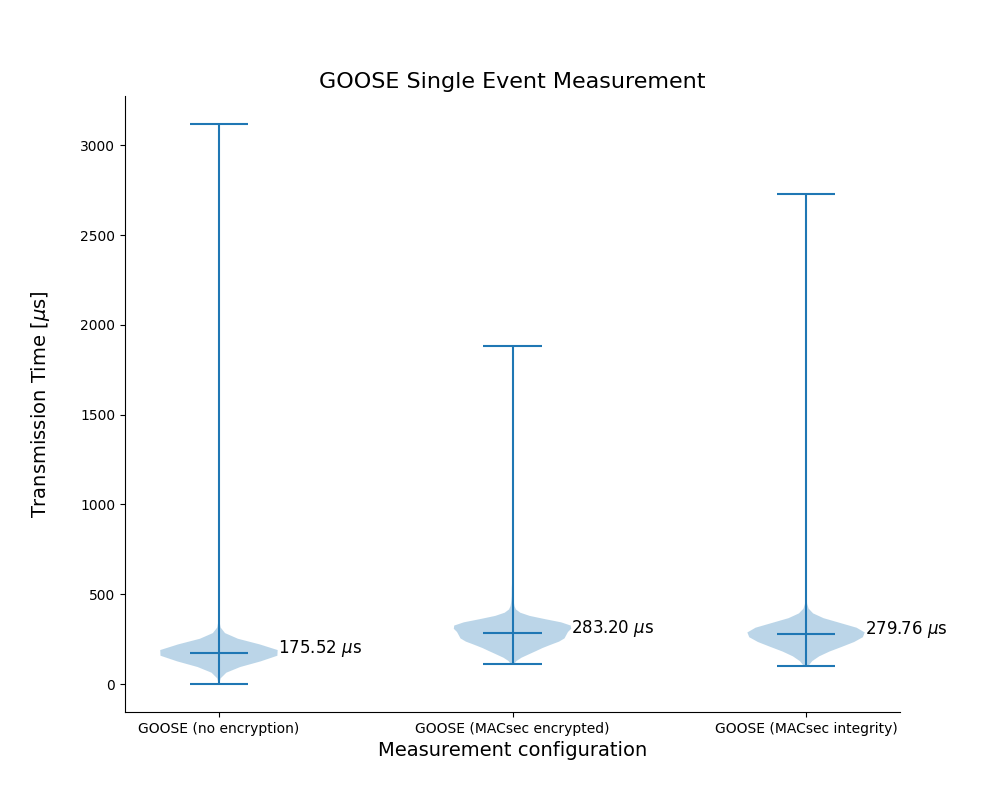
\includegraphics[width=\textwidth]{images/GOOSE_group_all_configs.png}
        \caption{Time comparison of a single GOOSE transmission}
        \label{imgae:GOOSETimings}
    \end{subfigure}
    \hfill
    \begin{subfigure}[b]{0.49\textwidth}
        \centering
        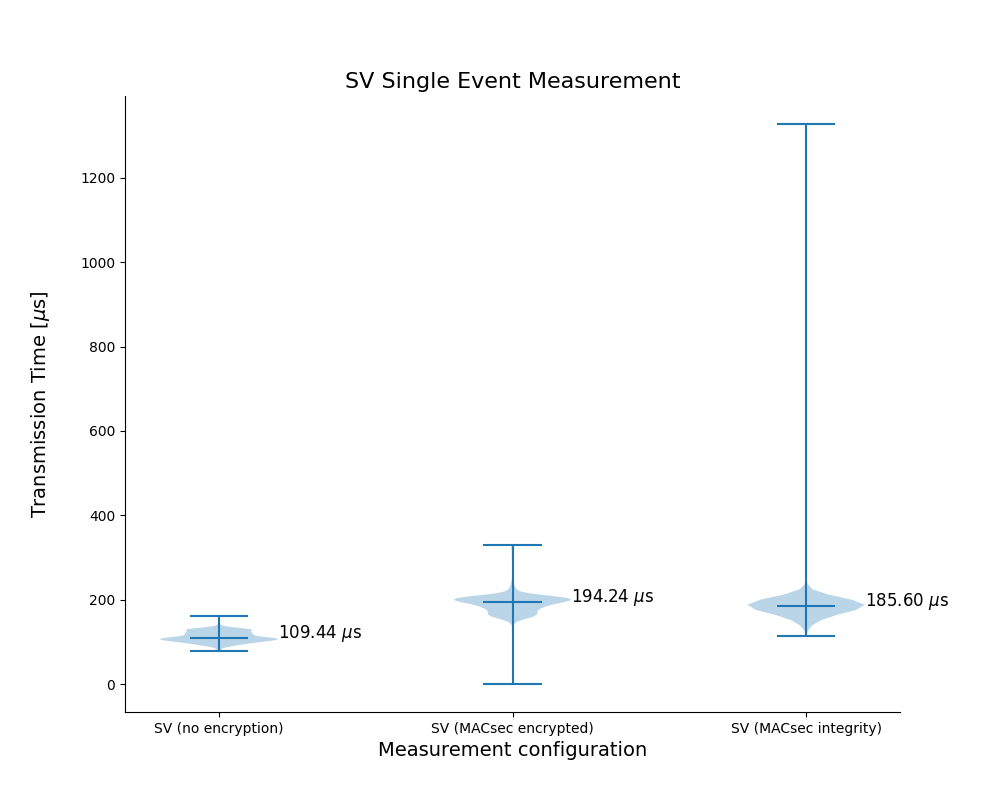
\includegraphics[width=\textwidth]{images/SV_group_all_configs.png}
        \caption{Time comparison of a single SV transmission}
        \label{image:SVTimings}
    \end{subfigure}
\end{figure}

\noindent As can be seen here, both Ethernet-based packets are transmitted in well below the IEC 61850 standard specification of 3 ms 
\cite{fixedLatencyGOOSESV:2021} regardless of the chosen configuration. Furthermore, securing the packets results in an extension of the transmission 
time of approximately 100 $\mu$s for both message types. It can be seen that activating the encryption in the AEAD cipher leads to a minimal 
increase in transmission time. This is likely due to the necessary rearrangement of the data payload into the Ethernet frame, which is not needed 
if only integrity checks are performed. Overall, the change in transmission times between these two configurations is nevertheless minimal at around 
6 $\mu$s for both message types. 

\subsection{Temporal Influence of MACsec on MMS messages}
\label{subchapter:EvalMMS}
\noindent For the MMS measurement, IED1 was configured to only perform the periodic update of the data points in the measurement unit of the internal 
SCL data structure. During this process, the time required for an MMS request-response sequence is measured on the client side. Since this message 
exchange involves two MMS messages, the resulting time is divided by two in the next step to determine the average transmission time. Identical to 
Chapter \ref{subchapter:EvalGOOSESV}, the measurement is then repeated 1000 times for all three configurations. The results of these measurements are 
displayed in Figure \ref{image:MMSTimings}. 

\begin{figure}[h]
    \centering
    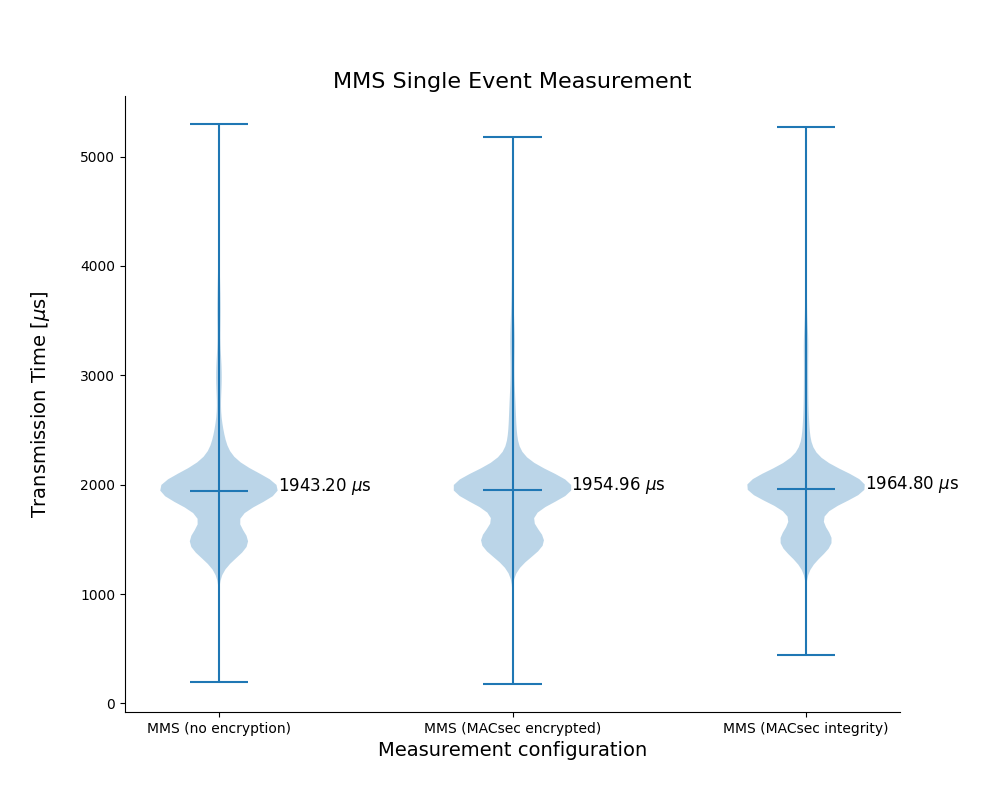
\includegraphics[width=0.55\textwidth]{images/MMS_group_all_configs.png}
    \caption{Time comparison of a single MMS transmission}
    \label{image:MMSTimings}
\end{figure}

\noindent As displayed in Figure \ref{image:MMSTimings}, the time measurements for MMS messages vary only marginally when compared to the transmission 
times of the Ethernet-based packets discussed in chapter \ref{subchapter:EvalGOOSESV}. This delay is likely due to the overhead caused by the additional 
processing in the higher layers of the OSI stack. Moreover, the time measurement for MMS transmission contains the application internal management of 
the SCL data structure in IED1, which further impacts the absolute transmission time of the measurements. However, the trend in the variance between 
the different test configurations is consistent with the other measurements, as the additional processing time for the MACsec protection of the frame 
is set to approximately 100 $\mu$s. Analog to GOOSE and SV, the IEC 61850 standard specifies a timing requirement for MMS packets of 100 ms 
\cite{fixedLatencyGOOSESV:2021}. As demonstrated in this measurement, the transmission time of MMS messaging with an active MACsec security module is 
well below the required time period. 

%%%%%%%%%%%%%%%%%%%%%%%%%%%%%%%%%%%%%%%%%%%%%%%%%%%%%%%%%%%%%%         Conclusion          %%%%%%%%%%%%%%%%%%%%%%%%%%%%%%%%%%%%%%%%%%%%%%%%%%%%%%%%%%%
\section{Conclusion}
\label{chapter:conclusion}
\noindent The aim of this paper was to investigate the extent to which the integration of MACsec in industrial communication would provide a viable 
alternative to the currently established security systems. In order to be able to evaluate this correctly, we implemented a test environment  
consisting of three IEDs, which can be configured to exchange the desired IEC 61850 messages. Going further, we evaluated, based on 
our measurement results, whether the timing and security requirements of the IEC 61850 and IEC 62351 standards can be considered fulfilled.  

\smallskip
With regard to the time requirements of the messages, Chapter \ref{chapter:evaluation} shows that all packets are transmitted in well below the required 
time periods. In addition to this, the measurements prove that the optionally activatable encryption of the AEAD cipher does not lead to a major increase 
in computational overhead. Therefore, confidentiality can be added to the security goals for all message types, regardless of the OSI model layer on which 
they operate. 

\smallskip
Only the IEC 62351 requirement mandating that a complete end-to-end security model for power systems shall be implemented \cite{Review_IEC62351:2019} cannot 
be fulfilled by MACsec. Due to the underlying architecture of this security standard, MACsec provides encryption of Ethernet-based packets, but must therefore 
be re-encrypted at each hop of the transmission. Other security standards such as TLS would fulfill this requirement, as they operate based on the TCP 
frame structure and can therefore be routed without a decryption of the message. However, simultaneously, packets below layer 4 of the OSI stack cannot 
be processed with TLS, which again would result in GOOSE and SV packets being transmitted unencrypted if implemented in a SAS. For this reason, we propose 
a hybrid implementation of both standards in a SAS for future work. In this scenario, MACsec could be used for LAN-internal communication security, while 
TLS provides the protection from a gateway component to external communication partners.    

%%%%%%%%%%%%%%%%%%%%%%%%%%%%%%%%%%%%%%%%%%%%%%%%%%%%%%%%%%%%%%       Acknowledgments       %%%%%%%%%%%%%%%%%%%%%%%%%%%%%%%%%%%%%%%%%%%%%%%%%%%%%%%%%%%
\section{Acknowledgments}
\noindent The presented work is part of the research project \emph{KRITIS Scalable Safe and Secure Modules} (KRITIS³M), which is funded by the Project 
Management Jülich (PtJ) and the German Federal Ministry for Economic Affairs and Climate Action (BMWK) under funding code 03EI6089A. Special thanks to 
Tobias Frauenschlaeger, Franziska Rasp and Peter Heller for their constructive feedback during the development of this paper.
%%%%%%%%%%%%%%%%%%%%%%%%%%%%%%%%%%%%%%%%%%%%%%%%%%%%%%%%%%%%%%     Begin of References      %%%%%%%%%%%%%%%%%%%%%%%%%%%%%%%%%%%%%%%%%%%%%%%%%%%%%%%%%%
\printbibliography
%%%%%%%%%%%%%%%%%%%%%%%%%%%%%%%%%%%%%%%%%%%%%%%%%%%%%%%%%%%%%%%%%%%%%%%%%%%%%%%%%%%%%%%%%%%%%%%%%%%%%%%%%%%%%%%%%%%%%%%%%%%%%%%%%%%%%%%%%%%%%%%%%%%%%%
\end{document}
